\documentclass[10pt, a4paper]{article}
\usepackage[utf8]{inputenc}
\usepackage{hyperref}
\usepackage{url}
\usepackage{graphicx}
\usepackage{caption}
\usepackage{multicol}
\usepackage{titlesec}
\usepackage{rotating}
\usepackage{threeparttable}
\usepackage{lipsum}
\usepackage{subcaption}
\usepackage{listings}               % for languages like C, Python
\usepackage{adjustbox}                % Balances the columns of the last page
\usepackage{balance}                % Balances the columns of the last page
\usepackage{booktabs}              % Nicer tables
\usepackage[capitalise]{cleveref}  % Clever references to stuff.
\usepackage[margin=1.2in]{geometry}
\usepackage[
    protrusion=true,
    activate={true,nocompatibility},
    final,
    tracking=true,
    kerning=true,
    spacing=true,
    factor=1100]{microtype}
\SetTracking{encoding={*}, shape=sc}{40}
\renewcommand{\familydefault}{\sfdefault}
\newcommand{\textFunc}[1]{\texttt{\textit{#1}}}
\newcommand{\textDef}[1]{\texttt{#1}}
\newcommand{\fig}[1]{Figure \ref{#1}}
\newcommand{\todo}{\textbf{TODO}}
\newcommand{\app}[1]{Appendix \ref{#1}}

%  Start Document

% \title{Software Engineering for Quadcopter Control \subtitle{CSE303}}
% \author{Vrushank Charan Agrawal }
% \author{Supervisor: Timothy Bourke }
% \date{October 2022}

\begin{document}
\setcounter{figure}{0}

\begin{figure}
    \centering
    \begin{subfigure}[b]{0.35\textwidth}
        \centering
        \includegraphics[width=\textwidth]{cool_logo.jpg}
        \label{Polytechnique}
    \end{subfigure}
    \label{Cool Logos}
\end{figure}

% \thispagestyle{plain}
\begin{titlepage}
    \vspace*{0.5cm}
    \begin{center}
        % \vspace{0.5cm}
        \Large
        \textbf{Software Engineering for Quadcopter Control}
        
        \vspace{0.5cm}
        \large
        CSE303 - Computer Science Project
            
        \vspace{2.0cm}
        \textbf{Author:} \text{Vrushank Agrawal}
        
        \vspace{0.5cm}
        \textbf{Supervisor:} \text{Dr. Timothy Bourke}
           
        \vspace{2.0cm}
        \textbf{Abstract}
    \end{center}
    A quadcopter (Unmanned Aerial Vehicle) is a naturally unstable embedded system that uses different control algorithms to guide its movement. Usually, quadcopters are programmed in languages like \textDef{C} or \textDef{C++} which are complex to directly use for understanding and composing reactive behaviours of embedded systems. In this report, we will study the Bitcraze Crazyflie 2.1 quadcopter and describe its static structure including main tasks and components of its feedback control loop. We will create a block diagram to study the dataflow between these different tasks to concretely understand its control algorithm and eventually analyze the possibility to reprogram it in a dataflow synchronous language like Lustre that offers an alternative and simpler approach to study control algorithms through high-level block diagrams.
    \vspace*{\fill}
\end{titlepage}
\clearpage

\tableofcontents
\clearpage

\section{Introduction}
    A quadcopter (a type of drone) is a four-propeller helicopter, usually arranged in a square, with four independent rotors. The need for aircraft with greater maneuverability and hovering ability has led to a rise in quadcopter research. The four-rotor design allows quadcopters to be relatively simple in design yet highly reliable and maneuverable, allowing them to be programmed for remote piloting by a ground control operator. Active research in the area is continuing to increase the abilities of quadcopters which are now used for various civil and military applications such as environment exploration, land surveys, photography, remote strike execution, etc. With further research, quadcopters would be capable of advanced autonomous missions that are currently not possible with other vehicles. \\

\begin{figure}[hbt!]
    \centering
    \begin{subfigure}[b]{0.28\linewidth}
    \rotatebox{90}{
            \centering
            \includegraphics[width=\linewidth]{back.jpg}
        }
        \caption{Bottom View.}
        \label{bottom}
    \end{subfigure}
    \hfill
    \begin{subfigure}[b]{0.35\textwidth}
        \centering
        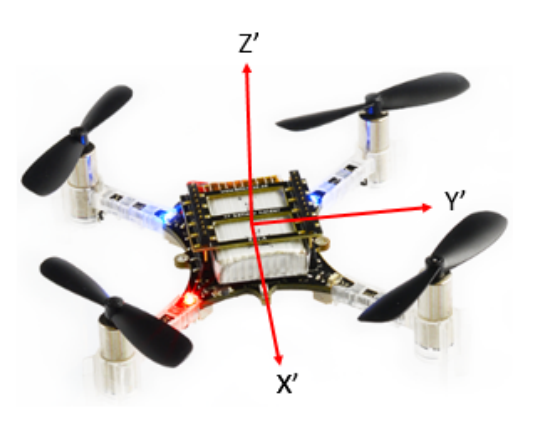
\includegraphics[width=\textwidth]{axes2.png}
        \caption{Axes}
        \label{axes}
    \end{subfigure}
    \hfill
    \begin{subfigure}[b]{0.31\textwidth}
        \rotatebox{180}{%
            \centering
            \includegraphics[width=\textwidth]{front.jpg}    
            }
        \caption{Top View}
        \label{axes}
    \end{subfigure}
    \caption{Crazyflie 2.1 quadcopter}
    \label{Crazyflie}
\end{figure}

    Quadcopters are usually written in languages like C/C++ that are complex and hard to use for replicating reactive behaviors of embedded systems. In this report we will study a quadcopter and analyze the possibility to replicate parts of its code in a dataflow synchronous language like Lustre where it is simpler to model and study reactive behaviours of embedded systems. We will use the Bitcraze Crazyflie 2.1 quadcopter which has been specifically developed for testing and research purposes shown in \fig{Crazyflie}. For the hardware, the crazyflie uses an ARM Cortex-M4, a $1$Mb flash, and the BMI$088$ 3 axis accelerometer/gyroscope and BMP$388$ high precision pressure sensor both manufactured by Bosch electronics \cite{bitcraze}.
    
\section{Design of Quadcopter}
    A quadcopter uses 4 propellers divided into 2 sets of diagonal pairs which rotate clockwise and anti-clockwise respectively. A pair of propellers on the same side spin in the opposite direction , i.e. diagonal propellers spin in the same direction. This is done to nullify the torque generated as a reaction of the upward force generated when the propellers rotate with some angular speed as shown in \fig{rotate}. A quadcopter has 6 degrees of freedom where 3 degrees are for transitional movement along the x, y, and z axes while 3 degrees are for rotational movement along x, y, and z axes termed roll, pitch, and yaw respectively as shown in \fig{rot_DOF} \cite{IIJEM}.
    
    \begin{figure}[hbt!]
        \centering
        \begin{subfigure}[b]{0.51\textwidth}
            \centering
            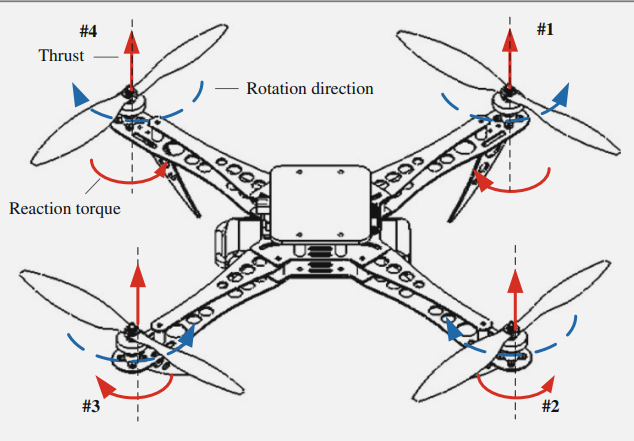
\includegraphics[width=\textwidth]{rotation.png}
            \caption{Propeller rotation}
            \label{rotate}
        \end{subfigure}
        \hfill
        \begin{subfigure}[b]{0.41\textwidth}
            \centering
            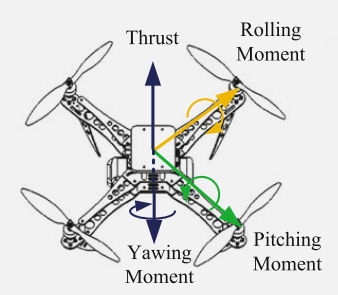
\includegraphics[width=\textwidth]{rot_dof.png}
            \caption{Rotational Degrees of Freedom}
            \label{rot_DOF}        
        \end{subfigure}
        \caption{Quadcopter Rotation and Degrees of Freedom \cite{book}}
        \label{DOF}
    \end{figure}
    
    \subsection{Movement}
    Even though a quadcopter has six degrees of freedom, the following four variables can be used to control its movements \cite{book} which have been illustrated in \fig{Movements}.

    \begin{itemize}
        \item \textDef{Thrust}: This is characterized as the transitional movement of the quadcopter along the z-axis or \textit{upward-and-downward movement} \cite{book}. This movement is controlled by changing the angular speed of the propellers by an equal amount as shown in \fig{Thrust}. Here, all motors change angular speed with the same amount and as a result, there is a net upward force on the quadcopter. So, for example, if the quadcopter needs to rise, the angular speed of the propellers will be increased proportionally to increase the upward force acting on it against the gravitational force pulling it downwards and vice-versa if it needs to fall.
        \item \textDef{Roll}: This is characterized as the rotational movement of the quadcopter along the x-axis or \textit{leftward-and-rightward movement} \cite{book}. So, for example, if the quadcopter wants to roll right, it would speed up motors on the left side ($\#3, \#4$) by some amount and slow down the two on the right ($\#1, \#2$) by the same amount as shown in \fig{roll}. Doing this creates an increased net force on the left side which lifts it on that side to produce a right roll.

        \item \textDef{Pitch}: This is characterized as the rotational movement of the quadcopter along the y-axis or \textit{forward-and-backward movement} \cite{book}. If the quadcopter wants to pitch forward, it speeds up the two motors at the back ($\#3, \#2$) and slows down the two at the front ($\#1, \#4$) as shown in \fig{pitch}. Doing this increases the torque at the back-end of the quadcopter and it rises up relative the inertial frame while generating a forward pitching movement
                
\begin{figure}[hbt!]
    \centering
    \begin{subfigure}[b]{0.41\textwidth}
        \centering
        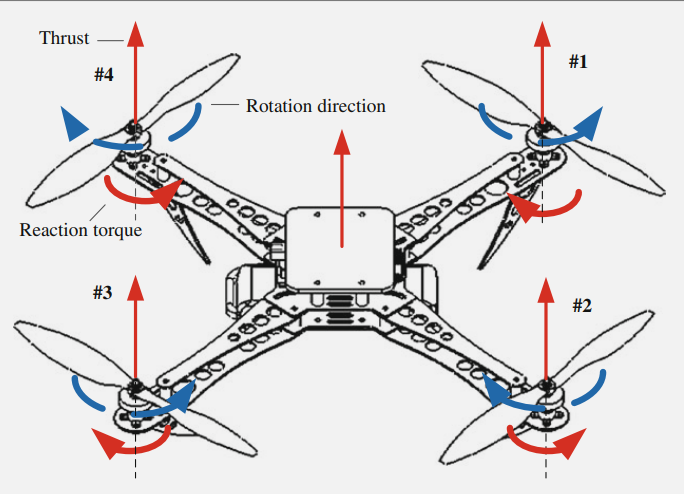
\includegraphics[width=\textwidth]{thrust.png}
        \caption{Upward Thrust}
        \label{Thrust}
    \end{subfigure}
    \hfill
    \begin{subfigure}[b]{0.45\textwidth}
        \centering
        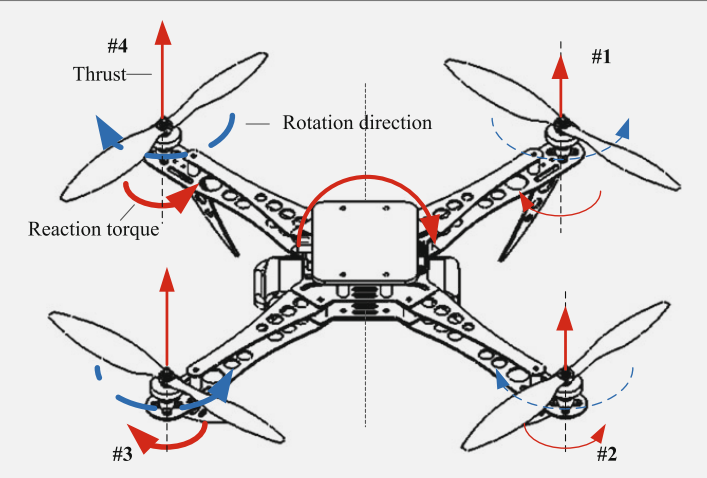
\includegraphics[width=\textwidth]{roll.png}
        \caption{Right Roll}
        \label{roll}        
    \end{subfigure}
    \hfill
    \begin{subfigure}[b]{0.45\textwidth}
        \centering
        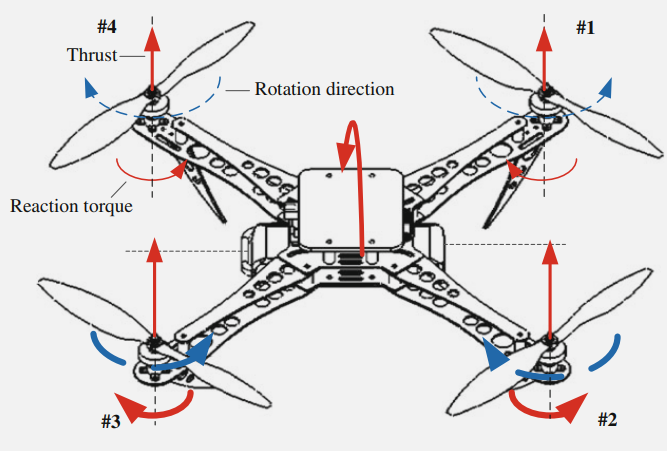
\includegraphics[width=\textwidth]{pitch.png}
        \caption{Forward Pitch}
        \label{pitch}        
    \end{subfigure}
    \hfill
    \begin{subfigure}[b]{0.41\textwidth}
        \centering
        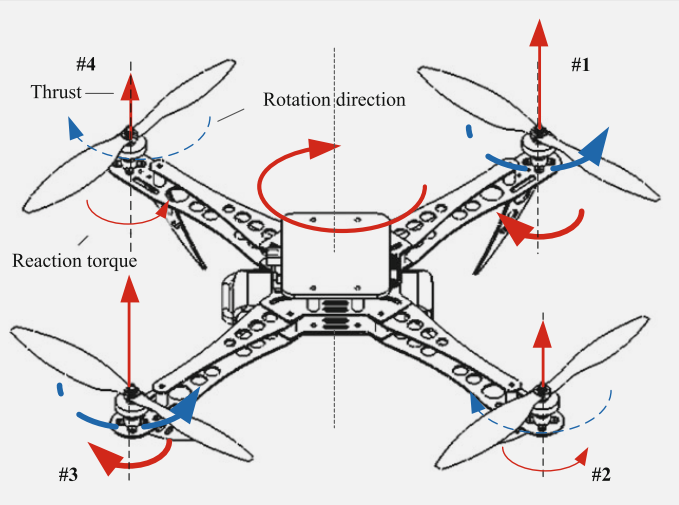
\includegraphics[width=\textwidth]{yaw.png}
        \caption{Clockwise Yaw}
        \label{yaw}        
    \end{subfigure}
    \caption{Quadcopter movements as a result of change in motor angular speeds \cite{book}.}
    \label{Movements}
\end{figure}

        \item \textDef{Yaw}: This is characterized as the rotational movement of the quadcopter along the z-axis or \textit{clockwise-and-anticlockwise movement}. This movement is realized by increasing and decreasing the angular speed of the diagonal propellers by the same amount. So, if the quadcopter wants to yaw clockwise, the angular speed of the propellers rotating clockwise ($\#4, \#2$) will be decreased while the angular speed of the propellers rotating anti-clockwise ($\#1, \#3$) will be increased by the same amount as shown in \fig{yaw}. A net unequal reactionary torque would be generated in the clockwise direction relative to the copter's z-axis hence turning it clockwise.
    \end{itemize}
    
    \subsection{Control Algorithms}
    Control algorithms are methods that let a quadcopter decide in real time which movements (described above) to use to reach its final destination (desired setpoint). Control algorithms are employed in a feedback loop mechanism where sensors provide data to the control algorithm that calculates the error between the current position, determined using the measured data, and the desired setpoint and then chooses the optimal movement to minimize the error while repeating the process until the desired setpoint is achieved. 
    \\ \\
    The Crazyflie 2.1 quadcopter software provides three different control algorithms--- PID (Proportional-Integral-Derivative), INDI (Incremental Nonlinear Dynamic Inversion), and Mellinger. The INDI and Mellinger controllers are direct applications of \cite{INDI} and \cite{Mellinger} which have only recently been integrated into the Crazyflie firmware without rigorous testing or documentation. The PID control algorithm, on the other hand, has been rigorously tested and widely documented in the firmware and is also a simple and standard algorithm hence, we will study it further.

    \subsubsection{PID Controller}
    The PID control algorithm is a linear algorithm that is widely used in robotics. It functions by calculating the error or difference between a measured output (sensors data) and a desired setpoint and adjusts the system control inputs such that the calculated error is corrected in a controlled manner in several loops to reach the desired set point to prevent sudden hiccups in the system. The PID algorithm consists of three control parameters,  P--Proportional, I–-Integral and D–-Derivative. The mathematical expression of the discrete-time PID algorithm is given as the following control function: $$u_p = K_pe(t) + K_d\frac{de(t)}{dt} + K_i \int_0^te(\tau)d\tau$$ Here, the term with $K_p$ determines the reaction to the current error (Proportional), the term with $K_i$ determines the reaction based on a sum of recent errors (Integral) while the term with $K_d$ responds to the rate at which the error has been changing (Derivative) \cite{IIJEM}. A block representation of a PID controller is show in \fig{PID block}.

\begin{figure}[hbt!]
    \centering
    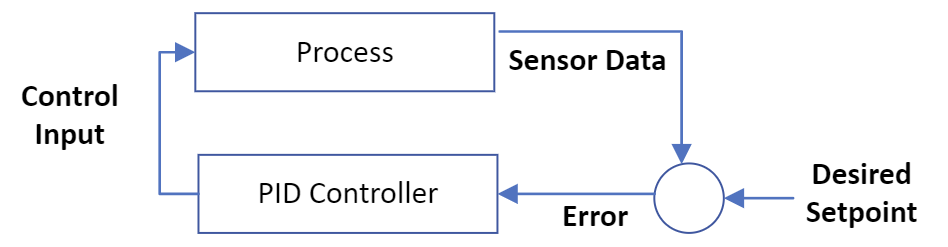
\includegraphics[width=0.81\textwidth]{pid_controller.png}
    \caption{Block diagram for a PID controller in a quadcopter's control loop.}
    \label{PID block}
\end{figure}

\section{Control in Crazyflie}
    The crazyflie 2.1 quadcopter uses the open-source FreeRTOS real-time operating system for its microcontroller \cite{bitcraze_freeRTOS} which is responsible for the real-time operations of the quadcopter.
    
    \subsection{Source Code}
    To study the crazyflie, we studied its code repository hosted on github \cite{firmware} that contains over $1000$ files and more than $375,000$ lines of code using tools like \textDef{CScope} and \textDef{CTags} that are specficially desgined to navigate large \textDef{C} code repositories. The root directory contained several subdirectories for \textDef{build, tests, tools, documentation, and vendor} (which contained code for third-party software integrations like FreeRTOS), but the main directory useful for our analysis was \textFunc{src} that contained the crazyflie source code. This \textFunc{src} directory contained subdirectories shown in \app{dirTree} for the expandable decks \cite{Decks} (\textFunc{decks}), sensors (\textFunc{drivers}), hardware abstraction layer (\textFunc{hal}), third-party libraries (\textFunc{lib}), stm32 integrated circuit for the microcontroller  (\textFunc{platform}) that are all used to support the main crazyflie code in the \textFunc{modules} subdirectory. 
    \\ \\
    The \textFunc{/src/modules} directory is divided into two subdirectories---\textFunc{interface} that contains all header files and \textFunc{src} that contains all \textDef{C} files. For our analysis, we stayed in the \textFunc{/src/modules/src} directory that contained all \textDef{C} source files for the feedback control loop (\textFunc{stabilizer.c}) and its five phases described below. The \textFunc{estimator.c} contained calls to estimator algorithms (\ref{estimator}), \textFunc{crtp\_commander.c} contained the \textDef{Commander} functions (\ref{commander}) and calls to other \textDef{C} files supporting the \textDef{Commander}'s functionalities, \textFunc{controller\_pid.c} contained functions for the PID controller (\ref{controller}), and \textFunc{power\_distribution\_quadrotor.c} contained functions for power distribution in the quadcopter's motors (\ref{motors}).

    \subsection{Tasks}
    A real time application can be structured as a set of independent tasks run by a scheduler where each task executes within its own context with no dependency on other tasks within the system or the scheduler itself. At any instant, the scheduler decides which task executes on the microcontroller. A task itself has no knowledge of the scheduler activity and it is the responsibility of the scheduler to ensure that the processor context (register values, stack contents, etc) when a task is swapped in is the same as when the same task was swapped out. This is achieved by providing individual stacks for each task \cite{freeRTOS}.
    \\ \\     
    Initially, we assumed that the control algorithm was divided into several individual tasks handled by the FreeRTOS scheduler. We thus searched for functions like \textFunc{xTaskCreate} and \textFunc{xTaskCreateStatic} in the crazyflie-firmware repository \cite{firmware} that are required to create tasks for handling by the scheduler \cite{xTask}. We retrieved the complete list of tasks created using \textFunc{xTaskCreate} and listed them in \app{a:xTask}. Out of these 21 tasks, 20 are for optional decks (that can be added to improve quadcopter's movement \cite{Decks}) while one is for led lighting sequence. None are directly related to the feedback control loop. For \textFunc{xTaskCreateStatic}, we used the classical \textDef{DEBUG PRINTING} method to check which functions are being called as static tasks when the crazyflie 2.1 is connected and flown and these have been listed in \app{a:xTaskStatic}. Out of the listed functions crteaed as static tasks, only \textFunc{stabilizerInit} and \textFunc{sensorsTaskInit} functions are directly related to the control loop, but both are implemented one after the other and do not switch amongst each other through semaphores during program execution. The \textFunc{estimatorKalmanTaskInit}, also related to the feedback control loop, is initialized but not ultimately used as the estimator defaults to the less computationally expensive \textFunc{estimatorComplementary} function instead. The \textFunc{sensorsTaskInit}, as the name suggests, is to retrieve information from the sensors and is not particularly useful for our analysis, and thus, we will only study the \textFunc{stabilizerInit} static task below.
    
    \subsection{Feedback Control Loop}
    The feedback control loop is the main loop of a quadcopter that constantly evaluates the quadcopter's position and plans its future trajectory using the control algorithms. The feedback control loop for the crazyflie 2.1 is initialized as the \textFunc{stabilizerInit} task that calls the \textFunc{stabilizerTask} function present in the \textFunc{stabilizer.c} file of its firmware repository. This control loop can be divided into five main phases namely: \textDef{Sensors, Estimator, Commander, Controller, Motors} that are explained below and have been drawn as a block diagram in \fig{block} representing the main data flow in the feedback control loop. In the diagram, the main \textDef{Drone Process} initiates the feedback control loop by calling the \textDef{Sensors} block which is followed until the \textDef{Motors} block that gives back control to the drone process to complete the loop.

\begin{figure}[hbt!]
    \centering
    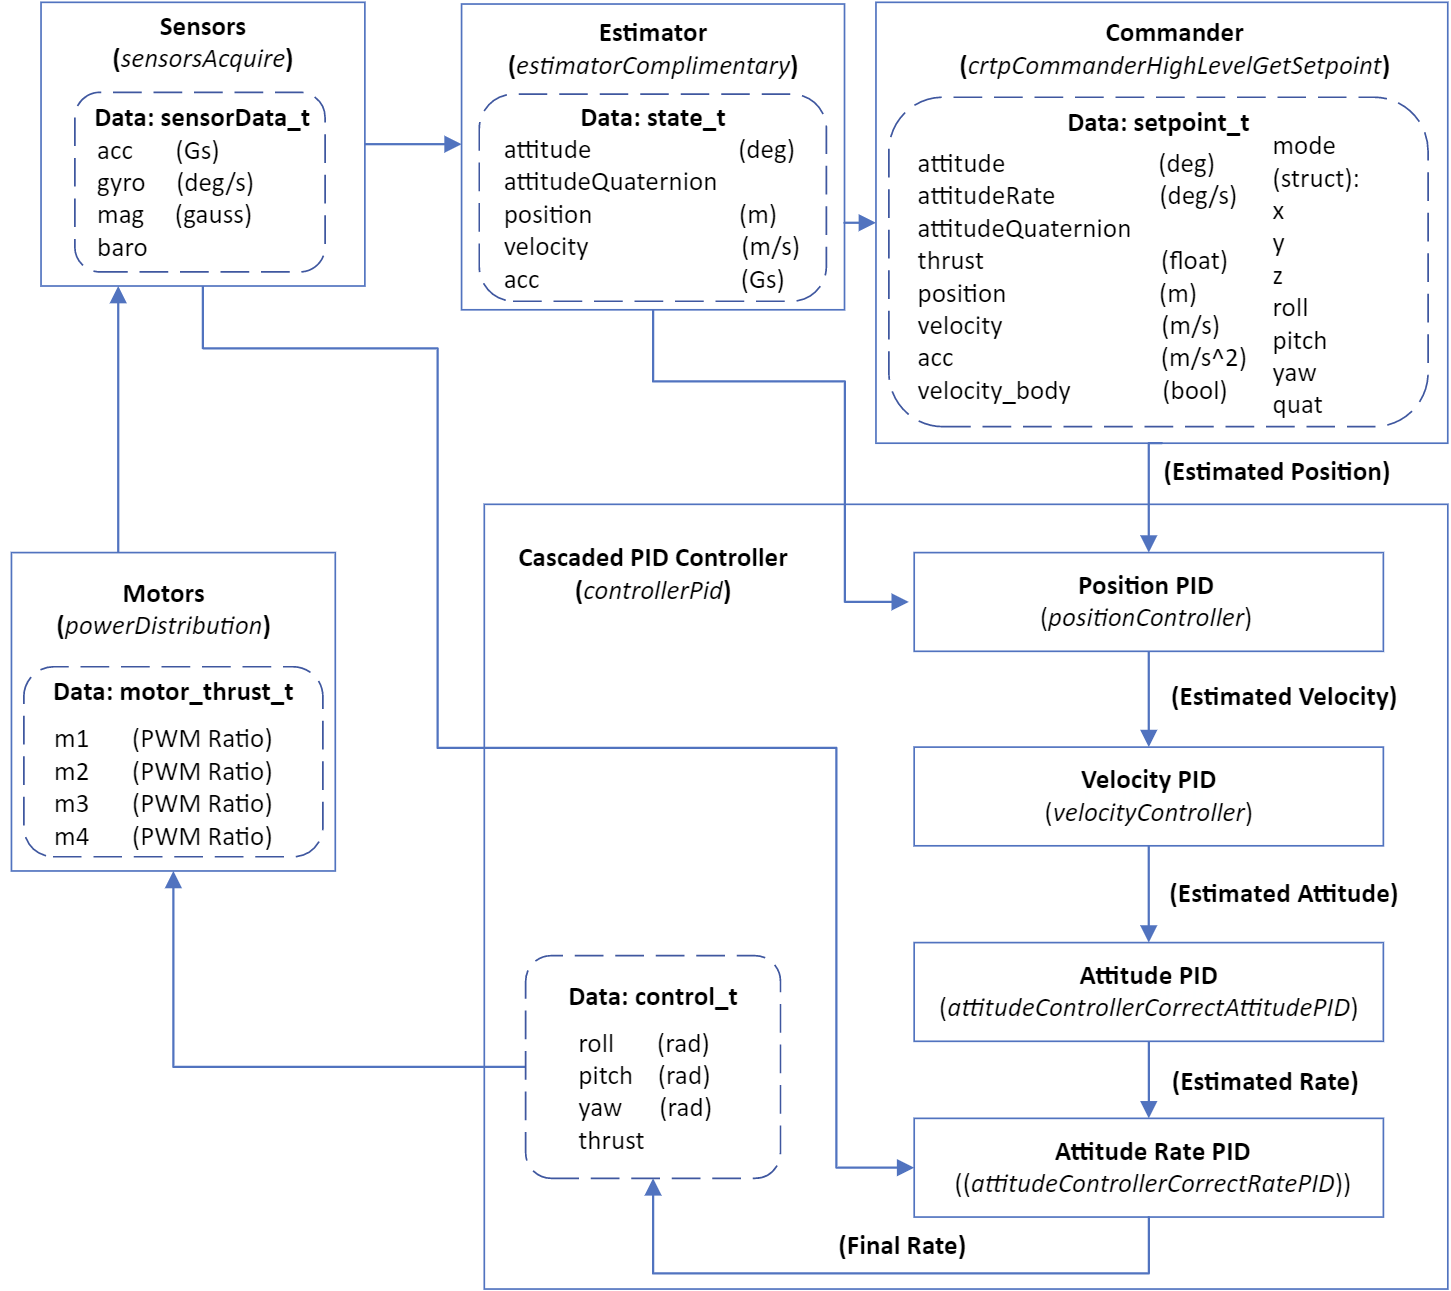
\includegraphics[width=0.9\textwidth]{main_block.png}
    \caption{Feedback control loop dataflow block diagram}
    \label{block}
\end{figure}

    \subsubsection{Sensors}
    \label{sensors}
        The crazyflie 2.1 uses two IMU (Inertial Measurement Unit) sensors BMI088 (3 axis accelerometer) and BMP388 (high precision pressure sensor). The control loop starts by first fetching data from the sensors through the \textFunc{sensorsAcquire} function in the following struct:
        \begin{lstlisting}[language=C]
    typdef struct sensorData_s {
        Axis3f acc;     // Gs
        Axis3f gyro;    // deg/s
        Axis3f mag;     // gauss
        Axis3f baro;
        uint64_t interruptTimestamp;
    } sensorData_t;
        \end{lstlisting}
        This data is sent to the \textDef{Estimator} and the \textDef{Controller} which use the readings as explained below.

    \subsubsection{Estimator}
    \label{estimator}
        The estimator is where the crazyflie uses one of three estimator algorithms (\textFunc{estimatorComplementary, estimatorKalman, or estimatorOutOfTree}) to decrease the noise in the sensors data and provide a better estimate of the state variables required by the control algorithm. The defualt estimator is \textFunc{estimatorComplementary} which uses the \textFunc{gyro} and \textFunc{acc} readings to calculate the attitude of the quadcopter at a rate of 250Hz. Attitude is a combination of \textDef{roll}, \textDef{pitch}, and \textDef{yaw}. The velocity component is updated using the \textFunc{acc} readings at the same frequency as attitude and the position readings are updated using the velocity readings at a frequency of 100Hz. The estimator algorithm also calculates \textFunc{attitudeQuaternion} but these are not yet used and are there for future integration in an improved state estimate. The crazyflie firmware uses the \textFunc{stateEstimator} function to access these algorithms and the final output is stored in the following struct:
        \begin{lstlisting}[language=C]
    typdef struct state_s {
        attitude_t attitude;    // deg
        quaternion_t attitudeQuaternion;
        point_t position;       // m
        velocity_t velocity;    // m/s
        acc_t acc;              // Gs
    } state_t;
        \end{lstlisting}
        This struct is passed to the \textDef{Commander} and the \textDef{Controller}.

    \subsubsection{Commander}
    \label{commander}
        The commander is where the quadcopter sets the desired destination setpoint. The crazyflie 2.1 uses  the \textFunc{crtpCommanderHighLevelGetSetpoint} function to evaluate the next setpoint. This function uses the \textFunc{plan\_current\_goal} function which has a \textFunc{planner} variable that keeps track of the setpoints of the trajectory in a \textFunc{traj\_eval} struct. The \textFunc{planner} uses the previous setpoint data to evalute the new setpoint and updates this new setpoint as the latest setpoint to be used for the next loop calculation. If the quadcopter is in an active trajectory, the new setpoint is updated using the \textFunc{commanderSetSetpoint} function otherwise it is not changed and current setpoint is nullified. Finally, if the setpoint is updated, then the \textFunc{commanderGetSetpoint} function fetches this latest setpoint to fly to in the following struct:
        \begin{lstlisting}[language=C]
    typdef struct setpoint_s {
        attitude_t attitude;     // deg
        attitude_t attitudeRate; // deg/s
        quaternion_t attitudeQuaternion;
        float thrust;
        point_t position;       // m
        velocity_t velocity;    // m/s
        acc_t acceleration;     // Gs
        bool velocity_body;     // true if velocity in body frame
        struct {
            stab_mode_t x;
            stab_mode_t y;
            stab_mode_t z;
            stab_mode_t roll;
            stab_mode_t pitch;
            stab_mode_t yaw;
            stab_mode_t quat;
        } mode;
    } setpoint_t;
        \end{lstlisting}
        This data structure is passed to the \textDef{Controller}.
 
    \subsubsection{Controller}
    \label{controller}
        The controller is the phase where the \textFunc{setpoint}, \textFunc{state}, and \textFunc{sensors} data generated in the previous three steps is used to calculate the appropriate thrust required by each motor to reach the desired setpoint. The controller can use any of the three controller algorithms (\textDef{PID}, \textDef{INDI}, and \textDef{Mellinger}) but as mentioned earlier, we will study \textDef{PID} and look at the \textFunc{controllerPid} function. This function uses the \textFunc{mode} variable from the \textFunc{setpoint} data struct that specifies if the quadcopter is static (\textDef{modeAbs}) or in flight (\textDef{modeVelocity}) to cap the desired \textFunc{yaw} between $-180^{\circ}$ and $180^{\circ}$ which might overflow this interval if the drone is in velocity mode when the \textFunc{attitudeRate} is regularly appended.
        \\\\
        The PID controller implemented in the crazyflie is actually a Cascaded PID controller which linearly evaluates \textDef{position}, \textDef{velocity}, \textDef{attitude}, and \textDef{attitudeRate} to eventually determine the thrust passed into motor power distribution. The PID controller constants ($K_p, K_i, K_d$) used in the crazyflie are given in \app{pidconst}. The \textDef{position} is evaluated by the \textFunc{positionController} function at a frequency of 100Hz when it runs the \textFunc{runPid} function to calculate the desired \textDef{velocity} which is updated in the \textFunc{setpoint}. The \textFunc{positionController} directly calls the \textFunc{velocityController} function (100Hz) which uses these recently updated \textDef{velocity} readings to evaluate the desired \textDef{attitude} by again using the \textFunc{runPid} function. Afterward, the \textFunc{attitudeControllerCorrectAttitudePID} function uses these recently calculated desired \textDef{attiude} readings with the previous readings from the \textFunc{state} struct to evaluate the desired \textDef{attitudeRate} readings. Finally, the \textFunc{attitudeControllerCorrectRatePID} function sets the desired \textDef{roll}, \textDef{pitch}, and \textDef{yaw} rate using the \textFunc{pidSetDesired} function and also uses \textFunc{gyro} readings from the \textFunc{sensors} struct to further precise the \textFunc{attitudeRate} readings even though they are not taken into account in the current implementation. The controller then updates the desired \textDef{rate} outputs in the following struct:
        \begin{lstlisting}[language=C]
    typdef struct control_s {
        int16_t roll;
        int16_t pitch;
        int16_t yaw;
        float thrust;
    } control_t;
        \end{lstlisting}
        which is passed to the \textDef{Motors}.
    
    \subsubsection{Motors}
    \label{motors}
        In this final phase of the loop, the \textFunc{powerDistribution} function uses the data from \textFunc{control} struct to calculate the appropriate thrust for each of the four motors and set their values in the following struct:    
        \begin{lstlisting}[language=C]
    typdef struct motors_thrust_s {
        int16_t m1;
        int16_t m2;
        int16_t m3;
        int16_t m4;
    } motors_thrust_t;
        \end{lstlisting}
        This struct is used by the \textFunc{motorsSetRatio} function to set the desired \textDef{thrust} for each motor. This step completes the loop which passes the control back to the \textDef{Drone Process} that runs the next iteration of the feedback control loop with the \textDef{Sensors} phase described in $3.2.1$.

% \section{Experiments}
% \todo

    
\section{Conclusion}
    In this report, we introduced quadcopters and studied in detail the Bitcraze crazyflie 2.1 to understand its control structure and the general dataflow. From the analysis, we located the feedback control loop in the \textDef{stabilizer.c} file implemented in the \textFunc{stabilizerTask} function. On further study, we discovered that this control loop runs in a simple linear fashion in a cyclic algorithm that executes each task one by one contrary to our initial assumption where the loop would have been divided into several FreeRTOS tasks running in parallel and communicating via semaphores. It would have been useful to have this information before starting the project as that would have saved us time studying the FreeRTOS functions. We would have used that time to perform experiments with the drone to further study its feedback control loop.
    % \\ \\
\section{Further Steps}
    The analysis provided in Section 3 and the block diagram in \fig{block} provide a promising first step for the gradual implementation of crazyflie's \textDef{C} code in a dataflow synchronous language like \textDef{Lustre} to study how much of a typical UAV controller can be rewritten in a block-diagram language. This is particularly useful for engineers who use dataflow synchronous languages (block diagram languages) to understand, describe, and compose reactive behaviours of embedded systems.

\begin{thebibliography}{10}

    \bibitem{bitcraze}
    Bitcraze, "Crazyflie 2.1",
    \textit{bitcraze.io:},
    https://www.bitcraze.io/products/crazyflie-2-1/.
    Accessed 28 November 2022.

    \bibitem{book}
    Quan, Quan. Introduction to Multicopter Design and Control. Springer Singapore, 2017. 1. pp.7-10.

    \bibitem{IIJEM}
    Ostojic, Gordana \& Stankovski, Stevan \& Tejic, Branislav \& Dukic, Nikola \& Tegeltija, Srdjan. (2015). Design, control and application of quadcopter. International Journal of Industrial Engineering and Management. 6. 43-48. 

    \bibitem{Fire_Ex}
    Manimaraboopathy, M. \& Christopher, H. \& Vignesh, S. \& selvan, P.. (2017). Unmanned Fire Extinguisher Using Quadcopter. International Journal on Smart Sensing and Intelligent Systems. 2017. 471-481. 10.21307/ijssis-2017-264.

    \bibitem{INDI}
    Smeur, Ewoud \& Chu, Q.P. \& Croon, Guido. (2015). Adaptive Incremental Nonlinear Dynamic Inversion for Attitude Control of Micro Air Vehicles. Journal of Guidance, Control, and Dynamics. 39. 1-12. 10.2514/1.G001490. 

    \bibitem{Mellinger}
    Mellinger, Daniel et al. “Trajectory generation and control for precise aggressive maneuvers with quadrotors.” The International Journal of Robotics Research 31 (2010): 664 - 674.
    
    \bibitem{bitcraze_freeRTOS}
    Bitcraze, "Adding a new system task",
    \textit{bitcraze.io},
    https://www.bitcraze.io/documentation/repository/crazyflie-firmware/master/development/systemtask/.
    Accessed 06 December 2022
    
    \bibitem{freeRTOS}
    FreeRTOS, "Tasks and Co-routines",
    \textit{freertos.org:},
    https://www.freertos.org/taskandcr.html.
    Accessed 29 November 2022.
    
    \bibitem{firmware}
    Github, "bitcraze/crazyflie-firmware",
    \textit{github.com},
    https://github.com/bitcraze/crazyflie-firmware/.
    Accessed 29 November 2022.

    \bibitem{xTask}
    FreeRTOS, "RTOS xTaskCreate",
    \textit{freertos.org},
    https://www.freertos.org/a00125.html.
    Accessed 29 November 2022.
    
    \bibitem{Decks}
    Bitcraze, "Expansion decks of the Crazyflie 2.X",\\
    \textit{bitcraze.io},
    https://www.bitcraze.io/documentation/system/platform/cf2-expansiondecks/.
    Accessed 03 December 2022

\end{thebibliography}
\clearpage

\appendix
\section{xTask Callers}
\subsection{Functions calling xTaskCreate}
\label{a:xTask}
\begin{multicols}{2}
    \begin{itemize}
        \item \textFunc{activeMarkerDeckInit}
        \item \textFunc{bigQuadInit}
        \item \textFunc{flowdeckInit}
        \item \textFunc{flowdeck2Init}
        \item \textFunc{gtgpsInit}
        \item \textFunc{lighthouseInit}
        \item \textFunc{drm1000Init}
        \item \textFunc{mrInit}
        \item \textFunc{oaInit}
        \item \textFunc{Init}
    \end{itemize}
\columnbreak
    \begin{itemize}
        \item \textFunc{uart1testInit}
        \item \textFunc{uart2testInit}
        \item \textFunc{usdInit}
        \item \textFunc{usdLogTask}
        \item \textFunc{zRangerInit}
        \item \textFunc{zRanger2Init}
        \item \textFunc{cpxInit}
        \item \textFunc{cpxExternalRouterInit}
        \item \textFunc{cpxUARTTransportInit}
        \item \textFunc{dtrStartProtocolTask}
        \item \textFunc{ledSeqInit}
    \end{itemize}
\end{multicols}

\subsection{Functions calling xTaskCreateStatic}
\label{a:xTaskStatic}
\begin{multicols}{2}
    \begin{itemize}
        \item \textFunc{pmInit}
        \item \textFunc{sysLinkInit}
        \item \textFunc{crtpserviceInit}
        \item \textFunc{logInit}
        \item \textFunc{memInit}
    \end{itemize}
\columnbreak
    \begin{itemize}
        \item \textFunc{paramInit}
        \item \textFunc{platformserviceInit}
        \item \textFunc{estimatorKalmanTaskInit}
        \item \textFunc{sensorsTaskInit}
        \item \textFunc{stabilizerInit}
    \end{itemize}
\end{multicols}
% \clearpage

\section{PID \textDef{Controller} constants}
\label{pidconst}
    \begin{multicols}{2}
    \subsection{Position Controller}
        \begin{itemize}
            \item X
            \begin{itemize}
                \item $K_p = 2.0$
                \item $K_i = 0.0$
                \item $K_d = 0.0$
            \end{itemize}
            \item Y
            \begin{itemize}
                \item $K_p = 2.0$
                \item $K_i = 0.0$
                \item $K_d = 0.0$
            \end{itemize}
            \item Z
            \begin{itemize}
                \item $K_p = 2.0$
                \item $K_i = 0.5$
                \item $K_d = 0.0$
            \end{itemize}
        \end{itemize}
    \columnbreak
    
    \subsection{Velocity Controller}
        \begin{itemize}
            \item $V_x$
            \begin{itemize}
                \item $K_p = 25.0$
                \item $K_i = 1.0$
                \item $K_d = 0.0$
            \end{itemize}
            \item $V_y$
            \begin{itemize}
                \item $K_p = 25.0$
                \item $K_i = 1.0$
                \item $K_d = 0.0$
            \end{itemize}
            \item $V_z$
            \begin{itemize}
                \item $K_p = 25.0$
                \item $K_i = 15.0$
                \item $K_d = 0.0$
            \end{itemize}
        \end{itemize}
    \end{multicols}
    \\ \\
    \begin{multicols}{2}
    \subsection{Attitude Controller}
        \begin{itemize}
            \item Roll
            \begin{itemize}
                \item $K_p = 6.0$
                \item $K_i = 3.0$
                \item $K_d = 0.0$
            \end{itemize}
            \item Pitch
            \begin{itemize}
                \item $K_p = 6.0$
                \item $K_i = 3.0$
                \item $K_d = 0.0$
            \end{itemize}
            \item Yaw
            \begin{itemize}
                \item $K_p = 6.0$
                \item $K_i = 1.0$
                \item $K_d = 0.35$
            \end{itemize}
        \end{itemize}
    \columnbreak
    
    \subsection{Rate Controller}
        \begin{itemize}
            \item Roll Rate
            \begin{itemize}
                \item $K_p = 250.0$
                \item $K_i = 500.0$
                \item $K_d = 2.5$
            \end{itemize}
            \item Pitch Rate
            \begin{itemize}
                \item $K_p = 250.0$
                \item $K_i = 500.0$
                \item $K_d = 2.5$
            \end{itemize}
            \item Yaw Rate
            \begin{itemize}
                \item $K_p = 120.0$
                \item $K_i = 16.7$
                \item $K_d = 0.0$
            \end{itemize}
        \end{itemize}
    \end{multicols}
% \clearpage

\section{\textFunc{/src/} sub-directory tree in the root folder}
\label{dirTree}
\begin{figure}[hbt!]
    \captionsetup{singlelinecheck = false, format= hang, justification=raggedright, font=footnotesize, labelsep=space}
    \begin{measuredfigure}
        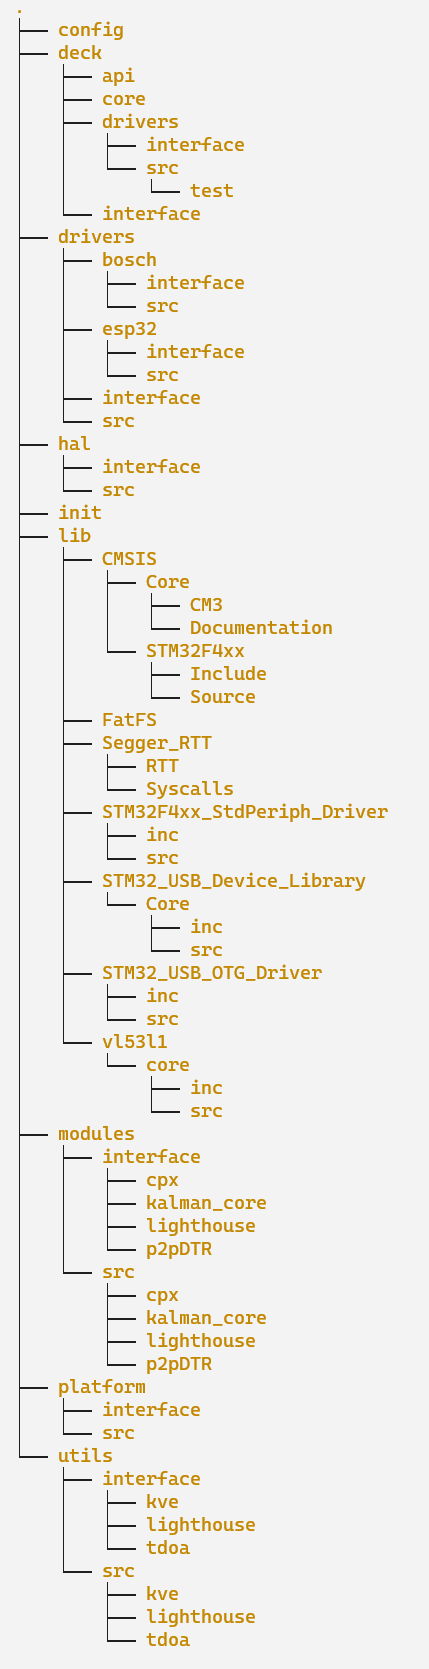
\includegraphics[width=0.205\textwidth]{directory_tree.png}
        \caption{\textFunc{/src/} tree}    
    \end{measuredfigure}
    \label{tree}
\end{figure}

\end{document}
